\noindent
\begin{tcolorbox}[colframe=black,width =7cm,colback=gray!20,arc=0pt]
\centering {\sc {\bf Questão 01}}
\end{tcolorbox}

Na figura abaixo temos $s(n) = A_c \cos(2 \pi f_c n)$, onde $f_c = \frac{1}{N}$, $N$ sendo o período da cossenoide.
Soma-se a $s(n)$ um ruído $\nu(n)$, branco, gaussiano e de densidade espectral de potência igual a $\frac{N_0}{2}$.
O sinal resultante $x(n)$ é filtrado por $H(f)$, um filtro passa-faixas ideal, de ganho unitário nos intervalos $[-f_c -\frac{W}{2}, -f_c + \frac{W}{2}]$ e $[f_c -\frac{W}{2}, f_c + \frac{W{2}}]$.
Na saída do filtro temos o sinal $y(n)$.

\begin{figure}[h!]
    \centering
    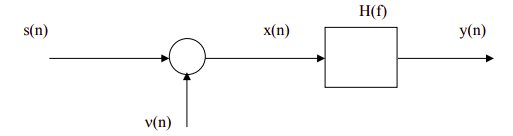
\includegraphics{../img/01/enunciado}
\end{figure}

Obtenha então e esboce:

\begin{enumerate}[label={\bf \alph*:},series=exerc,align=left]
    \item A densidade espectral de potência $S_y(f)$.
    A densidade espectral de potência do sinal após o filtro é dada por $S_y(f) = (S_x(f)+S_\nu(f))|H(f)|^2$, já que os sinais $x$ e $\nu$ são independentes.
    Como $x(n)$ é uma cossenoide, e $\nu(n)$ um ruído branco gaussiano, temos:
    \begin{equation*}
        S_y(f) = \begin{cases}
                      \frac{A_c^2}{4} + \frac{N_0}{2} \quad |f| = f_c \\
                      \frac{N_0}{2} \quad fc-\frac{W}{2} \leq |f| \leq f_c+\frac{W}{2} \text{ e } |f| \neq f_c \\
                      0 \quad \text{caso contrário}
                  \end{cases}
    \end{equation*}
    \item A função de autocorrelação $R_y(m)$.
    Podemos reescrever a densidade espectral de potência como:
    \begin{equation*}
        S_y(f) =
          \frac{N_0}{2}\mathrm{rect}(\frac{f-f_c}{W}) +
          \frac{N_0}{2}\mathrm{rect}(\frac{f+f_c}{W}) +
          \frac{A_c^2}{4}\delta(f-f_c) +
          \frac{A_c^2}{4}\delta(f+f_c)
    \end{equation*}
    Como sabemos que a função de autocorrelação é a Transformada de Fourier inversa da Densidade Espectral de Potência,
    \begin{equation*}
        R_y(m) = \mathcal{F}^{-1}\{S_y(f)\} = (\frac{A_c}{2}+N_0\mathrm{sinc}(Wm))\cos(2 \pi f_c m)
    \end{equation*}
    \item A função densidade de probabilidade da variável aleatória $y(n = N)$.

    Como $x(n)$ é um processo estocástico gaussiano, $y(n)$ também o é, com média $\mu_y(n) = \mu_x(n)H(0) = 0$ e variância $\sigma^2_y(n) = R_y(0) = \frac{A_c}{2} + N_0$.
    Logo, $y(n=N) \sim N(0, \frac{A_c}{2} + N_0)$.
\end{enumerate}
